\documentclass[10pt,twocolumn,letterpaper]{article}

\usepackage{cvpr}
\usepackage{times}
\usepackage{epsfig}
\usepackage{graphicx}
\usepackage{amsmath}
\usepackage{amssymb}
\usepackage{graphics}
\usepackage{subfigure}
\usepackage{amssymb}
\usepackage{amsthm}
\usepackage{amsmath}
\usepackage{algorithm}
\usepackage{algorithmic}
\DeclareMathOperator*{\argmin}{argmin}

% Include other packages here, before hyperref.

% If you comment hyperref and then uncomment it, you should delete
% egpaper.aux before re-running latex.  (Or just hit 'q' on the first latex
% run, let it finish, and you should be clear).
\usepackage[pagebackref=true,breaklinks=true,letterpaper=true,colorlinks,bookmarks=false]{hyperref}

% \cvprfinalcopy % *** Uncomment this line for the final submission

\def\cvprPaperID{1476} % *** Enter the CVPR Paper ID here
\def\httilde{\mbox{\tt\raisebox{-.5ex}{\symbol{126}}}}

% Pages are numbered in submission mode, and unnumbered in camera-ready
\ifcvprfinal\pagestyle{empty}\fi
\begin{document}

%%%%%%%%% TITLE
% \title{Fully Convolutional Attention Networks: Efficient Attention for Fine-Grained Recognition}
% \title{Fine-Grained Recognition with Automatic and Efficient Part Discovery}
% \title{Fine-Grained Recognition with Automatic and Efficient Visual Attention}
\title{Fine-Grained Recognition with Automatic and Efficient Part Attention}

\author{Xiao Liu, Tian Xia, Jiang Wang and Yuanqing Lin\\
Baidu Research\\
{\tt\small \{liuxiao12,xiatian,wangjiang03,linyuanqing\}@baidu.com}
}

\maketitle
%\thispagestyle{empty}

%%%%%%%%% ABSTRACT
\begin{abstract}
Fine-grained recognition is challenging due to the subtle local inter-class differences versus the large intra-class variations such as poses.
A key to address this problem is to localize discriminative parts to extract pose-invariant features.
However, ground-truth part annotations can be expensive to acquire.
Moreover, it is hard to define parts for many fine-grained classes.
This work introduces \textbf{Fully Convolutional Attention Networks (FCANs)}, a reinforcement learning framework to optimally glimpse local discriminative regions adaptive to different fine-grained domains.
Compared to previous methods, our approach enjoys four advantages:
1) the three components including feature extraction, visual attention and fine-grained classification are unified in an end-to-end system;
2) the weakly-supervised reinforcement learning procedure requires no expensive part annotations;
3) the fully-convolutional architecture speeds up both training and testing;
4) the greedy reward strategy accelerates the convergence of the learning.
% it is capable of simultaneous focusing its glimpse on multiple visual attention regions.
% Feng: I am not sure this is an advantage
We demonstrate the effectiveness of our method with extensive experiments on four challenging fine-grained benchmark datasets, including Stanford Dogs, Stanford Cars, CUB-200-2011 and Food-101.
\end{abstract}

\section{Introduction}
Fine-grained recognition refers to the task of distinguishing sub-ordinate categories, such as bird species~\cite{bd6}, dog breeds~\cite{bd4}, car models~\cite{bd5}, flower categories~\cite{NilsbackZ08,CuiZLB16}, food dishes~\cite{BossardGG14,ZhouL16}, etc.
With the great potential in rivaling human experts, it has shown tremendous applications in real world ranging from e-commerce~\cite{Bala15,KiapourHLBB15} to education~\cite{KumarBBJKLS12,BergLLAJB14}.
% Although great success have been achieved for basic-level recognition in the last few years, fine-grained recognition still faces two challenges.
Although great success has been achieved for basic-level recognition in the last few years~\cite{KrizhevskySH12,bd7,he2015deep}, fine-grained recognition still faces two challenges.
First, it is more difficult and time-consuming to gather a large amount of labeled fine-grained data because it calls for experts with specialized domain knowledge.
In addition, the difference between fine-gained classes is very subtle.
The most discriminative features are often not based on the global shape or appearance variation but contained in the mis-alignment of local parts or patterns.
For instance, as shown in Fig.~\ref{fig:teaser}, the eye texture and beak shape are crucial to differentiate between Parakeet Auklet and Rhinoceros Auklet.

\begin{figure}
\begin{center}
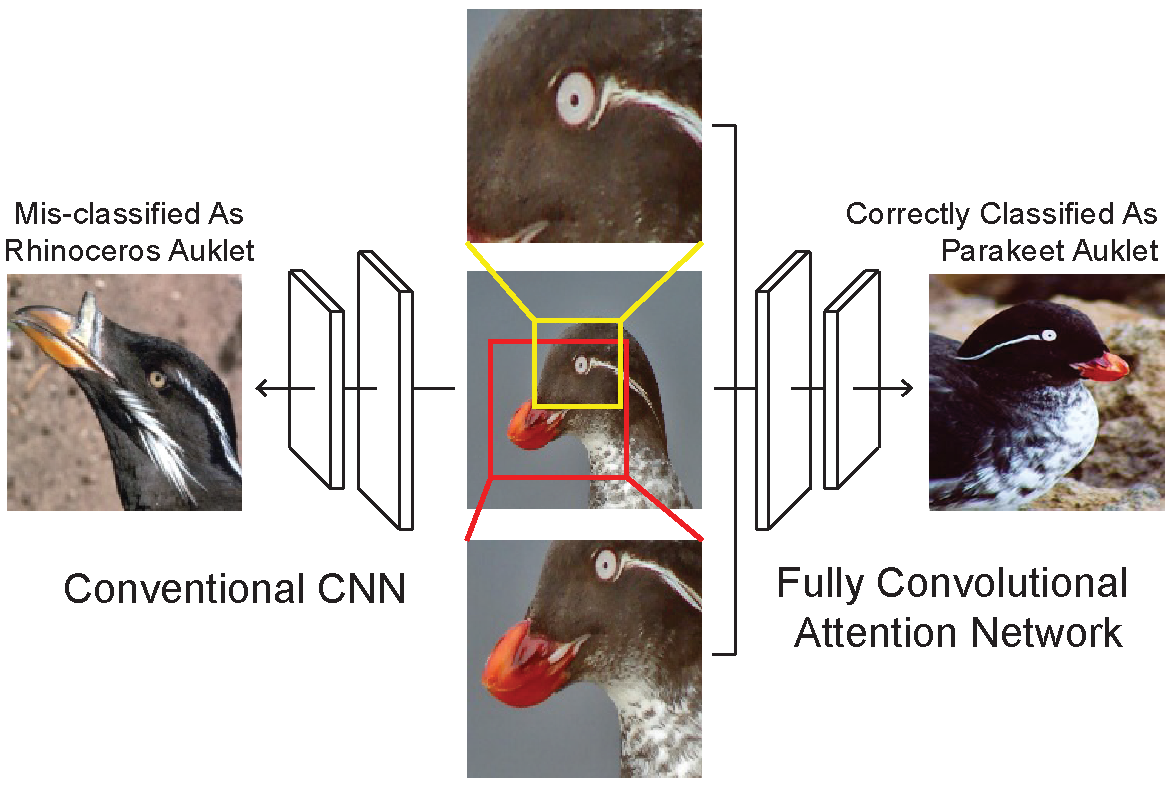
\includegraphics[width=.5\textwidth]{figs/teaser_v2.pdf}
\end{center}
\caption{Conventional CNN approach (left) finds difficulty in differentiating similar fine-grained categories with subtle local variations (eg., Rhinoceros Auklet against Parakeet Auklet).
In contrast, our proposed fully convolutional attention networks (right) is able to automatically and efficiently localize parts (eg., bird's eye and beak) given only weakly supervised fine-grained class labels.
}
\label{fig:teaser}
\end{figure}

\setlength{\tabcolsep}{0.5pt}
\begin{figure}[t]
\begin{center}
\begin{tabular}{ccc}
\includegraphics[height=0.25\linewidth,width=0.25\linewidth]{figs/hooded_oriole} &
\includegraphics[height=0.25\linewidth,width=0.4\linewidth]{figs/bmw} &
\includegraphics[height=0.25\linewidth,width=0.3\linewidth]{figs/kungpao_chicken} \\
\vspace{2pt}
Hooded Oriole & BMW & Kungpao Chicken \\
\includegraphics[height=0.25\linewidth,width=0.25\linewidth]{figs/scott_oriole} &
\includegraphics[height=0.25\linewidth,width=0.4\linewidth]{figs/benz} &
\includegraphics[height=0.25\linewidth,width=0.3\linewidth]{figs/yuxiang_rousi} \\
Scott Oriole & Mercedes-Benz & Yuxiang Rousi \\
(a) Bird & (b) Car & (c) Food
\end{tabular}
\end{center}
\caption{Fine-grained recognition often involves part localization, i.e. (a) localizing head and breast to distinguish birds, and (b) localizing brand to classify car makes.
It is relatively easy to define parts for structured objects like birds and cars.
However, it is hard to define rigid parts for unstructured classes, such as (c) food.
This may be solved by attention models.
}
\label{fig:teaser2}
% \vspace{-8pt}
\end{figure}

To that end, the main body of previous research has focused on devising more discriminative features by detecting and aligning object parts.
Nevertheless, most conventional methods~\cite{bd10,bd15} utilize manually defined parts to localize the regions, such as ``the head of a bird'', for fine-grained recognition.
Relying on manually defined parts has several drawbacks:
1) The precise part annotations are usually expensive to acquire.
2) The strongly supervised part-based model might fail if some parts are occluded.
3) For some fine-grained categories, it is very difficult to manually define parts for them.
For example, it is very difficult to define parts for food recognition, as suggested in Fig.~\ref{fig:teaser2}.
4) Most importantly, there is no clue that manually defined parts are optimal for all fine-grained recognition tasks.

To overcome these problems, we propose a visual attention framework called {\em Fully Convolutional Attention Networks} (FCANs) for fine-grained recognition without part annotation.
Given only image label, our framework utilizes reinforcement learning to simultaneously localize object parts and classify the object within the scene.
Intuitively, the framework simulates human visual system that proceeds object recognition via a series of {\em glimpse} on object parts.
At each glimpse, it strives to find the most discriminative location that can differentiate object's category given the previous observations.
%Similar to previous visual attention model~\cite{bd1,bd3}, we employ the REINFORCE algorithm~\cite{bd20}, where the location of each glimpse is an action, the image and the location of the previous glimpses are the state, and the reward measures the classification correctness.
Similar to previous visual attention models~\cite{bd1,bd3}, we employ the REINFORCE algorithm during training~\cite{bd20}, where the action is the location of each glimpse, the state is the image and the locations of the previous glimpses, and the reward measures the classification correctness.
The whole framework can be trained end-to-end and it is driven only by an image classification loss, thus requiring no manual part annotations.
The visual attention approach is demonstrated to perform well on fine-grained recognition without requiring manually labeled object parts~\cite{bd3}.

Compared to the previous reinforcement learning-based visual attention frameworks~\cite{bd1,bd3}, the FCANs enjoy better computational efficiency as well as higher classification accuracy in fine-grained recognition.
More concretely, our proposed framework improves the attention models in three ways:
\begin{itemize}
\item{\bf Computational Efficiency:} The previous frameworks run a convolutional neural network individually on each image crop, which is computationally expensive during both training and testing.
In contrast, our method re-uses the same feature maps (computed by a fully convolutional neural network~\cite{bd7,bd8}) during each glimpse in a way similar to Fast-RCNN~\cite{girshick2015fast}.
This makes training and prediction computationally more efficient because of the fully convolutional neural network architecture and feature sharing technique.
\item{\bf Multiple Part Localization:} During testing, our model is able to simultaneously locate multiple parts of adaptive sizes, while the previous frameworks~\cite{bd1,bd3} generally only locate one part at each iteration.
\item{\bf Fast Training Convergence:} Instead of assigning a delayed reward at the end of attention iterations as previous methods~\cite{bd7,bd8}, we apply a new greedy reward strategy at every step of attention, which is crucial to both the convergence speed of training and the accuracy of prediction.
\end{itemize}
% As a result, our proposed approach outperforms state-of-the-art reinforcement learning-based approaches~\cite{bd1,bd3} in fine-grained recognition accuracy by a large margin.
% It is also more suitable for larger datasets, which is common in industrial applications, because of its computational efficiency.

% The experiments demonstrate that the proposed framework can  significantly improve the performance over state-of-the-art reinforcement learning based methods without utilizing external data or complicated model fusion techniques.
% Note that we improve the previous state-of-the-art on Stanford Dogs from $82.6\%$ to $84.1\%$.

% We conduct extensive experimental evaluation on four fine-grained benchmark datasets: Stanford Dogs~\cite{bd4}, Stanford Cars~\cite{bd5}, CUB-200-2011~\cite{bd6} and Food-101~\cite{cvpr_ref1}.
As a result, our proposed approach improves the recognition accuracy over state-of-the-art reinforcement learning based methods~\cite{bd1,bd3} while being computationally more efficient. On Stanford Dogs, for example, we improve the previous state-of-the-art from 82.6\% to 84.2\% and decrease the prediction time from 250ms to 150ms on a single GPU.

% The remainder of the paper is organized as follows. The related work is reviewed in Section 2.
% The architecture of fully convolutional attention network is described in Section 3.
% The training process of the proposed framework is described in Section 4.
% The implementation details, performance studies, and experimental analysis are illustrated in Section 5.
% The conclusion and future work is presented in Section 6.

\section{Related Work}
Fine-grained recognition has been extensively studied in the computer vision literature.
We review the three most relevant directions in this section.

\subsection{Representation Learning}
Since the seminal work of AlexNet~\cite{KrizhevskySH12}, we are witnessing a fast-pacing transition from hand-crafted feature to end-to-end convolutional neural networks in representation learning.
Most of the current state-of-the-art fine-grained recognition algorithms are also based on deep CNN representation to distinguish the subtle difference.
Branson et al.~\cite{bd15} claim that integrating lower-level layer and higher-level layer features learns more discriminative representation for fine-grained recognition.
Lin et al.~\cite{bd16} propose a bilinear architecture to model local pairwise feature interactions for fine-grained recognition, where convolutional features from two models are combined in a translation invariant manner.
Qian et al.~\cite{bd17} propose a multi-stage metric learning framework to learn a distance metric that pulls data points of the same class close and pushes data points from different classes far apart.
Wang et al.~\cite{bd19} combine saliency-aware object detection approach and object-centric sampling scheme to extract more robust and discriminative features for large-scale fine-grained car classification.
In parallel to these efforts, our method combines representation learning with part detection in a unified framework that can be trained end-to-end.

\subsection{Part Models}
Since 70's, early cognitive research study~\cite{Rosch76} has shown that subordinate-level recognition is based on comparing the appearance details of object parts.
Drawing inspiration from this fact, various pose normalization methods~\cite{FarrellOZMDD11,ZhangFID13,ZhangPRDB14,bd10,bd11} have been proposed to focus on the important regions.
However, these methods are strongly supervised ones, heavily relying on manually pre-defined parts modeled by Poselet~\cite{BourdevM09} or DPM~\cite{FelzenszwalbGMR10}.
Due to this limit, most of recent efforts were spent on how to automatically discover critical parts in a weaker setting.
For instance, Berg et al.~\cite{bd9} use data mining techniques to learn a set of intermediate features that can differentiate two classes based on the appearance of a particular part.
Yang et al.~\cite{bd12} propose a template model to discover the common geometric patterns of object parts and the co-occurrence statistics of the patterns.
Similarly, Gavves et al.~\cite{bd13} and Chai et al.~\cite{bd14} segment images and align the image segments in an unsupervised fashion.
The aligned image segments are utilized for feature extraction separately.
Recently, Simon and Rodner~\cite{bd28} propose neural activation constellations, an approach that is able to learn part models in an unsupervised manner.
Compared to our method, however, these methods are not end-to-end trainable and require tedious and ad-hoc tuning of individual components.

% Zhang et al.~\cite{bd11} utilize part-based R-CNNs as whole-object and part detectors to detect the pose of the objects.
% The CNN appearance representation is then pose-normalized for fine-grained recognition.

% Some other works that find discriminative parts in an unsupervised way.
% Feng: in my opinion, data-mining already included unsupervised

\subsection{Attention Models}
One of the main drawbacks of part-based models is the need for a strong motivation in part definition (either by hand or by data-mining method), which may lack for many non-structured objects such as food dishes.
On the other hand, several works introduce attention-based models for task-driven object/part localization.
For instance, Mnih et al.~\cite{bd1} present a recurrent neural network model for object detection by adaptively selecting a sequence of attention regions and extract appearance representations in these regions.
Since this model is non-differentiable, it is trained with reinforcement learning technique to learn task-specific policies.
Ba et al.~\cite{bd2} extend~\cite{bd1} and successfully achieve good results on a more challenging multi-digit recognition task.
Despite the remarkable contributions in theory, the recurrent attention models still suffer from several drawbacks in practice.
First, they only result in small performance improvement.
For instance, Sermanet et al.~\cite{bd3} further extend~\cite{bd2} to fine-grained recognition but only achieve 76.8\% mean accuracy percentage (with 3 glimpses) on Stanford Dogs dataset while the result of GoogLeNet~\cite{bd7} baseline is 75.5\%.
Second, the computational burden is high.
Calculating features at each glimpse in~\cite{bd3} requires forwarding GoogLeNet three times, leading to very slow training and testing.
% In contrast, our proposed framework improves the attention models in two ways:
% \begin{itemize}\vspace{-8pt}
% \item {\bf Computational Efficiency:} It is much more computationally efficient because of the fully convolutional neural network architecture and feature sharing % technique.
% \item {\bf Multiple Part Localization:} It is capable of localizing multiple parts with different sizes simultaneously.
% \end{itemize}
% As a result, the proposed framework not only achieves noticeable improvements over state-of-the-art methods on several benchmark datasets,
% it is also more suitable to be applied to larger datasets, which is common in industrial applications, because of its computational efficiency.
An exceptional work is spatial transformer networks~\cite{jaderberg2015spatial}, which build on a differentiable attention mechanism that does not need reinforcement learning for training.
As an alternative approach, we show reinforcement learning can still be effective and efficient in improving fine-grained recognition.

% Compared to previous approaches, have remarkable contributions to fine-grained recognition problem,
% because they can learn the part localization and discriminative representation in an end-to-end way, and they do not require manually labeled object parts.

% \begin{itemize}
% \item \textbf{Small performance improvement.}~\cite{bd3}  achieves 76.8\% mean accuracy percentage (with 3 glimpses) on Stanford Dogs dataset while the result of GoogLeNet~\cite{bd7} baseline is 75.5\%. Considering the attention-based model is much more complicated, the improvement is slight.

% \item \textbf{High computational burden.}~\cite{bd3} employs GoogLeNet for representation learning. However, calculating the features at each glimpse requires forwarding GoogLeNet three times, leading to very slow training and testing.

% %\item \textbf{Convergence difficulty.} Because the attention-based models\cite{bd1,bd2,bd3} are trained with reinforcement learning, the convergence of the model is slow and heavily depends on the exploration parameters.
% \end{itemize}

% In contrast to the above works, the training and testing of the proposed work is much faster, and the recognition accuracy significantly outperforms the baseline methods.

\section{Fully Convolutional Attention Networks}

% \begin{figure*}[t]
% \begin{center}
% \includegraphics[width=6.8in]{1.pdf}
% \end{center}
% \caption{The architecture of the attention network. In this example, the attention network finds two parts of different sizes (the blue region and the yellow region).
% The upper part shows the architecture for testing, and the lower part shows the architecture for training. In testing, each part is resized to high resolution for classification. In training, the corresponding convolutional features in attention network is re-used for classification.}
% \label{fig:architecture}
% \vspace{-8pt}
% \end{figure*}

\begin{figure*}[t]
\begin{center}
\includegraphics[width=\linewidth]{figs/1-cropped.pdf}
\end{center}
\caption{The architecture of our FCANs framework.
In this example, the attention network finds two parts of different sizes (the blue region and the yellow region).
The upper part shows the architecture for testing, and the lower part shows the architecture for training.
During testing, we crop the corresponding part patches from the high resolution image for classification.
During training, we re-use the corresponding convolutional features in the attention networks for classification.
% Note that in practice, we compute all part attentions simultaneously by combing all the attention networks into a single fully convolutional network.
Note that in practice, we can compute all part attentions simultaneously.
This makes both training and testing computationally efficient.
}
\label{fig:architecture}
\vspace{-8pt}
\end{figure*}

% Conventional CNN methods compute features from the global appearance of an image, which is limited for discriminating classes in fine-grained domain.
% This section proposes fully convolutional framework, which enhances CNN augmented with part attention.
% Unlike previous part-based models~\cite{FarrellOZMDD11,ZhangFID13,ZhangPRDB14,bd10,bd11}, however, our method requires no manual annotation and can be trained in a unified network.
Fig.~\ref{fig:architecture} illustrates the architecture of the Fully Convolutional Attention Networks (FCANs) with three main components: the feature component, the attention component, and the classification component.

\textbf{Feature Map Extraction:}
The feature component contains a fully convolutional network that extracts features from the input image and its subsequent attention crops.
These feature maps are shared for both part attention and fine-grained classification.
During experiment, we adopt one of the popular CNN architectures (e.g., VGG-16~\cite{bd8}, GoogLeNet~\cite{bd7} or ResNet~\cite{he2015deep}) as the basis fully convolutional network, pre-trained on ImageNet dataset~\cite{bd19} and fine-tuned on the target fine-grained dataset.
During testing, the image and all attention crops are resized to a canonical size before feature extraction, similar to~\cite{bd1}.
Hence the amount of computation it performs can be controlled independently of the input image size.

During training, although cropping local image regions can achieve good performance, it requires us to perform multiple forward and backward passes of a deep convolutional network in one batch, where the time complexity for feature extraction depends on the number of parts and number of attention regions sampled for each part.
In practice, this is too time-consuming.
Thus, we extract feature maps from the original image at multiple scales and re-use them across all time steps.
The features for each part is obtained by selecting the corresponding region in the convolutional feature maps, so that the receptive field of the selected region is the same as the size of the part.
As a result, we only need to run the forward pass once in one training batch.

\textbf{Fully Convolutional Part Attention:}
The attention component localizes multiple parts by generating multiple part score maps from the basis convolutional feature maps.
Each score map is generated using two stacked convolutional layers and one spatial softmax layer.
The first convolutional layer uses 64 $3\times3$ kernels, and the second one uses one $3\times3$ kernels to output a single-channel confidence map.
The spatial softmax layer converts the confidence map into probability.
During testing, the model selects the attention region with the highest probability as the part location.
During training, the model samples attention regions multiple times according to the probability map.
The same process is applied for a fixed number of time steps for multiple part locations.
Each time step generates the location for a particular part.
We will detail this step in the following sections.

\textbf{Fine-Grained Classification:}
The classification component contains a convolutional network for each part as well as the whole image.
The classification network for each part is a fully convolutional layer followed by a softmax layer.
Different parts might have different sizes, and a local image region is cropped around each part location according to its size.
% We train an image classifier for each local image region as well as the whole image separately.
The final prediction score is the average of all the prediction scores from the individual classifiers.
In order to discriminate the subtle visual differences, each local image region is cropped at high resolution.

%The classification network in each step is a fully convolutional layer followed by a softmax layer, which uses the attention maps of all the parts in the last time step as well as the convolutional features of the whole image as the input.

% A  deep convolutional neural network is trained for each part for classification separately.

% During inference, we first localize multiple attention regions by selecting the location with the highest probability for each part in the attention network.
% We then zoom in on each part's location by resizing the regions around it to its corresponding high resolution.
% Each resized part region as well as the original image makes the prediction individually using the classification part.
% The final prediction score is the average of the prediction scores from the original image and all the attention regions.

\subsection{Model}
The entire attention problem is formulated into a Markov Decision Process (MDP).
During each time step of MDP, the FCANs work as an agent to perform an action based on the observation and receives a reward.
In our work, the action corresponds to the location of the attention region, the observation is the input image and the crops of the attention regions and the reward measures the quality of the classification using the attention region.
The target of our learning is to find the optimal decision policy to generate actions from observations, characterized by the parameters of the FCANs, to maximize the sum expected reward across all time steps.
% We introduce the mathematical notations below.

We define the input image as $x$ and the feature component computes the feature maps as $\phi(x)$.
The attention component outputs $T$ attention regions $\{a^1, \ldots, a^T\}$ with each region $a^t \sim \pi(a^t | \phi(x))$, where $\pi$ is the policy for attention selection.
At time step $t$, the classification component crops an image region $x(a^t)$, extracts a new feature $\phi(x(a^t))$ and predict classification score $s_t$.
It then computes the final class probability $y_t$ as the average of all prediction scores until time $t$
\begin{equation}
y_t = \frac{1}{t} \sum_{i=1}^t s_i(\phi(x(a^i)))
\end{equation}
The reward $r^t$ for the $t$-th step measures how $y_t$ matches the ground truth label $\hat{y}$.

% \textbf{Observation:} At each time step $t \in \{1, \ldots, T\}$, the agent receives an observation from the environment in the form of an image $x^t$.
% In our work, we feed $x^t$ with the same input image $x$.
% This makes observations the same across all time steps.

% \textbf{State:} For each step $t$, the agent maintains an internal state representation $s^t$ which summarizes information extracted from the history of past observations.
% In our model, $s^t$ is the feature pyramid extracted from the feature component.
% Since all observations are the same, the states also share the same representation.

% \textbf{Action:} The action corresponds to the attention region selection.

% Given the feature pyramid as state $s$, the attention component uses $T$ different fully convolutional networks to localize $T$ different parts, by generating a probability map $P(a^t | \phi, \theta^t_a)$ for each part at every time step $t$ ($t \in \{1, \ldots, T\}$).
% $a^t$ specifies the location (attention) of the $t$-th part.
% During inference, we select $a^t$ with the highest probability as the $t$-th part location.
% During training, we sample $a^t$ according to the probability map.
% $\theta_a = \{\theta^1_a, \ldots, \theta^T_a\}$ are the parameters for the $T$ attention networks.

% \textbf{Reward:} The reward $r$ measures the quality of the classification using the attention region.
% A straightforward reward strategy is to measure the final classification correctness.
% To avoid delayed reward, we design a {\em greedy reward} strategy and describe in section~\ref{sec: reward}.

\subsection{Training}

Since there are no ground-truth annotations to indicate where to select attention regions and each attention is a non-differentiable function, we adopt reinforcement learning to learn the network parameters.

Given a set of training images with ground truth labels $(x_n, \hat{y}_n)_{n=1\cdots N}$, we jointly optimize the three components to maximize the following objective function:
\begin{equation}
\max_{\theta} J(\theta) =  \max_{\theta_f, \theta_a, \theta_c} R(\theta_f, \theta_a) - \lambda L(\theta_f, \theta_c)
\end{equation}
where $\theta = \{\theta_f, \theta_a, \theta_c\}$ are the parameters of the feature networks, the attention networks and the classification networks respectively.
$\lambda$ is a balance weight.
\begin{equation}
L(\theta_f, \theta_c) = \frac{1}{NT} \sum_{n=1}^N \sum_{t=1}^T L^t_n(x_n, \hat{y}_n, \theta_f, \theta_c)
\end{equation}
is the average cross-entropy classification loss over $N$ training samples and $T$ time steps.
% Notice that we employ an approximated part classification method that is similar to Fast-RCNN~\cite{girshick2015fast} during training.
\begin{equation}
R(\theta_f, \theta_a) = \frac{1}{NT} \sum_{n=1}^N \sum_{t=1}^T E_{\theta}[r^t_n]
\end{equation}
is the average expected reward over $N$ training samples and $T$ time steps.
\begin{equation}
E_{\theta}[r^t_n] = \sum_{a^t_n} \pi(a^t_n|x_n, \theta_f, \theta^t_a) \ r(a^t_n)
\end{equation}
is the expected reward of the $t$-th selected attention region from the $n$-th sample.
$\theta^t_a$ is the parameters of the $t$-th attention network,
$x_n$ is the n-th input image, and $a^t_n$ is the $t$-th selected region.
$\pi(a^t_n|x_n, \theta_f, \theta^t_a)$ is the probability of selecting $a^t_n$ as the attention region.
The reward function $r(a^t_n)$ is crucial for developing an efficient learning algorithm. We describe the design of the reward function in the following section.

\subsection{Reward Strategy} \label{sec: reward}

A straightforward reward strategy is to measure the quality of the attention region selection policy as a whole using the final classification result, i.e., $r(a^t_n) = 1$ if $t=T$ and $y^t_n=\hat{y}_n$, and 0 otherwise.
Although MDP with such a reward strategy can learn in a recurrent way~\cite{bd1}, it confuses the effect of the selected regions in different time steps,
and it might lead to the problem of convergence difficulty.

We consider an alternative reward strategy, namely {\em greedy reward}:
\begin{equation}
r(a^t_n)=\left\{
\begin{array}{cc}
1 & t = 1 \ \wedge \ y^1_n = \hat{y}_n \\
1 & t > 1 \ \wedge \ y^t_n = \hat{y}_{n} \ \wedge \ L^t_n < L^{t-1}_n \\
0 & otherwise \end{array}
\right.
\end{equation}
where $y^t_n$ is the predicted classification result, $\hat{y}_n$ is the ground-truth label, and $L^t_n$ is the classification loss for the $n$-th sample at $t$-th step. If the image is classified correctly in the first step, the attention network immediately receives a reward. In other steps, we reward the corresponding attention network only if the image is classified correctly and the classification loss decreases with regards to the last time step.
Otherwise, the attention network receives zero reward.

Since the attention network immediately receives a reward when an image is correctly classified with the current attention region, the convergence of training is much easier.

\subsection{Optimization}

\begin{figure}[t]
\begin{center}
\subfigure[Forwarding]{
\includegraphics[scale = 0.4]{figs/2-1-revised.pdf}}
\hspace{0.05in}
\subfigure[Back-propagation]{
\includegraphics[scale = 0.4]{figs/2-2-revised.pdf}}
\end{center}
\caption{The forward (a) and back-propagation (b) processes for training attention networks as MDPs.
The dashed lines indicate the sampling procedures.
}
\label{fig:optimization}
\end{figure}

It is difficult to directly compute the gradient of $E_{\theta}[r^t_n]$ over $\theta$ because it requires evaluating exponentially many possible part locations during training.
Hence we employ REINFORCE algorithm and approximate the gradient in a Monte Carlo way~\cite{bd20}.

% To simply the notation, we define
% \begin{equation}
% \pi^t_n(\theta)  = \pi(a^t_n | x_n, \theta_f, \theta^t_a)
% \end{equation}
% and according to~\cite{bd20}
% \begin{equation}
% \nabla_{\theta} \left(\pi^t_n(\theta)\ r(a^t_n)\right) = \pi^t_n(\theta)\ \nabla_{\theta} \log \pi^t_n(\theta)\ r(a^t_n)
% \end{equation}
% Thus,
% \begin{eqnarray} \label{eq:policy_gradient}
 %\nabla_{\theta} E_{\theta}[r^t_n] = \sum_{a^t_n} \pi^t_n(\theta)\ \nabla_{\theta} \log \pi^t_n(\theta)\ r(a^t_n) \\
% \approx \frac{1}{K} \sum_{k=1}^K \nabla_{\theta} \left(\log \pi(a^t_{nk} | x_n, \theta_f, \theta^t_a)\right) r(a^t_{nk}) \nonumber
% \end{eqnarray}
\begin{equation}
\nabla_{\theta} E_{\theta}[r^t_n] \approx \frac{1}{K} \sum_{k=1}^K \nabla_{\theta} \left(\log \pi(a^t_{nk} | x_n, \theta_f, \theta^t_a)\right) r(a^t_{nk})
\label{eq:policy_gradient}
\end{equation}
where $a^t_{nk}\sim \pi(a^t_n | x_n, \theta_f, \theta^t_a) $ is sampled according to a multinomial distribution parameterized by the output confidence map of the $t$-th attention network.

The forward process of training the attention networks as MDPs is shown in Fig.~\ref{fig:optimization}. Given the basis convolutional feature maps $\phi(x)$ as input, the attention networks output the confidence map $\pi^t(\phi)$ for different time step. Each $\pi^t(\phi)$ forms a multinomial distribution, and the location of attention region $a^t$ is sampled under the distribution. The sampling procedure is repeated for $K$ times. We then use them for classification $c(a^t)$ and further get the reward $r(a^t)$.

During back-propagation, the gradient $\nabla_{\theta} L(\theta_f, \theta_c)$ can be  obtained by back-propagating the classification networks.
The gradient $\nabla_{\theta} R(\theta_f, \theta_a)$ is calculated using policy gradient as shown in Equation~\ref{eq:policy_gradient}.
Notice that when the reward is 0, we can just ignore the sample.

\subsection{Implementation Details}

\textbf{Step-wise training:} Although jointly training the entire model is possible, we develop a 3-step algorithm for the sake of training speed.
In the first step, we initialize and fine-tune the CNN model to extract the basis convolutional feature maps for attention and classification.
In the second step, we fix and cache the basis convolutional feature maps from the first step, and train the attention networks separately.
In the third step, we fix and cache the selected attention regions from the second step, and fine-tune the final classification model.
Through feature caching, repeated feature calculating is avoided.
Notice that the convolutional neural networks for attention and the final classification is different, though they are initialized similarly during pre-training described below.
We repeat these steps several times until convergence.

\textbf{Fast-RCNN approximation:} During training, although we can compute a multi-scale feature maps to obtain the features for high resolution region crops. It could still be time-consuming when the image resolution is large.
Thus, we employ an approximated feature extraction method that is similar to Fast-RCNN~\cite{girshick2015fast}, where we only compute a feature map from the input image at one scale.
The convolutional features for each part is obtained by selecting the corresponding region in the convolutional feature map of the whole image, so that the receptive field of the selected region is the same as the size of the part.
This further accelerates the training of attention networks.

Note that since we adopt a 3-step training, the Fast-RCNN approximation are only utilized during attention network training.
The final classification networks are still trained given the features extracted from cropped high resolution images.

% \subsection{Discussion}

% Our attention component is inspired from the recurrent visual attention model~\cite{bd1}.
% However, instead of building a recurrent attention network that share parameters over different time steps, our model uses multiple convolutional networks with different parameters to model the temporal effect.
% During testing, these attention networks work like independent part detectors that share the same basis image feature.
% It is even possible to combine all the attention networks into a single convolutional network to compute part attentions simultaneously.
% This makes inference much faster.

% Although we use fixed size and aspect ratio, learning part size and aspect ratio is also possible by using multiple ROI pooling operations with different sizes and aspect ratios at a location.
% The optimal size and aspect ratio at each location can be selected via a channel-wise max pooling operation.
% As a result, our method can be applied to attention regions with any aspect ratio.
% However, it increases the complexity of the model and the difficulty of convergence.

%Our method can also extend to learn a flexible number of parts.
%As pointed in~\cite{bd1}, our model can be augmented with an additional action that decides when it stops taking extra attention.
%This could be used to learn a cost-sensitive classifier by giving the agent a negative reward for each attention it takes, forcing it to trade off making correct classifications with the cost of taking more attentions.
%However, our experiments show that usually the benefit of attentions stops after 2-3 time steps.

%Finally, although our model is designed without part annotation.
%Adding part supervision into our framework is also straightforward.
%This can be done, for example, by adding intermediate supervision to the attention networks and train the whole system as multi-task learning.
%We leave this as future work.

\section{Experiments}

\begin{table}[t]
% \small
\begin{center}
\begin{tabular}{c|c|c|c|c|c}
\hline
Dataset & \ \#class \ & \ \#train \ & \ \#test \ & \ bbox \ & \ part \ \\\hline\hline
Stanford Dogs~\cite{bd4} \ & 120 & 12,000  &  8,580 & $\surd$ &    \\
Stanford Cars~\cite{bd5} \ & 196 & 8,144  & 8,041 & $\surd$ &  \\
CUB-200-2011~\cite{bd6} \ & 200 & 5,994 & 5,794 & $\surd$ & $\surd$ \\
Food-101~\cite{cvpr_ref1} \ & 101 & 75,750 & 25,250 & $ $ & $ $ \\\hline
\end{tabular}
\caption{Statistics for the four fine-grained benchmark datasets.}
\label{tab:statistics}
%\vspace{-20pt}
\end{center}
\end{table}

We conduct extensive experiments on four benchmark datasets, including Stanford Dogs~\cite{bd4}, Stanford Cars~\cite{bd5}, CUB-200-2011~\cite{bd6} and Food-101~\cite{cvpr_ref1}.
Table~\ref{tab:statistics} shows the statistics of the four datasets.

\subsection{Experimental Setup}

For Stanford Dogs dataset, we use the VGG-16 network~\cite{bd8} for feature extraction.
During pre-training, we first scale all images to $256 \times256 $ resolution, and fine-tune the VGG-16 net with randomly cropped $224\times224$ patches.
For each input image, the VGG-16 net outputs a $512\times16\times16$ \texttt{conv5\_3} feature map.
We then use the feature map to train the attention networks to find two parts.
The first part selects a $4\times4$ region in the feature map (corresponding to a $64\times64$ patch in the original image), and the second one selects a $8\times8$ region (corresponding to a $128\times128$ patch in the original image).
We then crop the two result attention patches and resize to $256\times256$ to train VGG-16 prediction models in the final classification stage.

We use different experimental settings for the Stanford Cars and CUB-200-2011 datasets because most previous methods on them take higher resolution inputs.
Specifically, we resize the input images to $512\times512$.
To enable larger training batch, we use GoogLeNet~\cite{bd7} to extract the convolutional features.
For each input image, GoogLeNet outputs a $512\times16\times16$ \texttt{inception\_5b/output} feature map.
We then train the attention networks to select $4\times4$ and $8\times8$ attention regions in the feature map.
During final classification, we resize the attention regions and the original images to $448\times448$ for prediction.
We use $12\times12$ average pooling for GoogLeNet to fit higher resolution inputs.

For the Food-101 dataset, we use ResNet-50~\cite{he2015deep} to extract the features of \texttt{res\_5c} layer.
The other settings are the same as in the experiments of Stanford Cars and CUB-200-2011.

We use RMSProp with mini-batch size 512, initial learning rate 0.01 and sampling number per step 16.

\subsection{Comparison with State-of-the-Arts}

We compare our framework with previous state-of-the-art methods and summarize the results from Table~\ref{tab:dog} to Table~\ref{tab:food}.

On Stanford Dogs, our model achieves a new state-of-the-art result (84.2\%) without using ground-truth bounding box or part annotations.
% Gavves et al.~\cite{bd13} utilize ground-truth bounding boxes during training and testing, but the results is only $50.1\%$.
% Karuse et al.~\cite{bd21} achieves $82.6\%$ accuracy at the expense of using additional web-data from Google Image Search.
% Simon and Rodner~\cite{bd28} learn part models in a completely unsupervised manner and achieve $68.1\%$ accuracy.
% Zhang et al.~\cite{bd27} select useful parts from multi-scale part proposals in objects, and use them to compute a global image representation for categorization. The accuracy is $79.9\%$.
Note that Sermanet et al.~\cite{bd3} use reinforcement learning based recurrent attention models, which is similar to our approach.
Our method improves them by more than 7\%, suggesting the FCANs as a more effective reinforcement learning framework for fine-grained recognition.

On Stanford Cars and CUB-200-2011, our recognition accuracy is competitive against previous methods.
Karuse et al.~\cite{bd21} achieve a higher 92.8\% accuracy on Stanford Cars at the expense of using additional web-data from Google Image Search.
Among all the methods that use the same set of training data, Lin et al.~\cite{bd16} obtain the highest recognition accuracy.
However, they pay the cost of constructing high dimensional bilinear feature vectors, which makes training and testing extremely slow, preventing its application for large-scale dataset.
Although our accuracy is lower than Lin et al.~\cite{bd16}, we use much less time for training and testing.
%Jaderberg et al.~\cite{jaderberg2015spatial} achieve an accuracy of 84.1\% without using bounding boxes, but it uses a strong Inception network as a baseline (82.3\% accuracy).
%We find using a similar baseline network, our algorithm can achieve state-of-the-art accuracy 84.3\% accuracy with two attention parts (spatial transformer uses 4 parts).

% Karuse et al.~\cite{bd21} achieves $92.8\%$ accuracy and Lin et al.~\cite{bd16} achieves $91.3\%$ without using bounding boxes.
% Although the result of the proposed method is not the best one on this dataset, it is simpler to implement than~\cite{bd21} and uses less time for training and testing than~\cite{bd16}.

% Xu et al.~\cite{bd23} use additional web data for training and achieve slight higher performance ($0.3\%$) than the proposed method.
% Lin et al.~\cite{bd16} obtains the highest recognition accuracy (85.1\%) at the cost of constructing high dimension bilinear feature vectors, which makes the training procedure extremely slow and limits its application for larger dataset.

On Food-101, our method sets a new recognition record, outperforming the second best method by more than 7\%.

\begin{table}[t]
\centering
\begin{tabular}
{c||c|c}\hline
Method &  bbox & Acc(\%) \\\hline\hline
% VGG-16   &  & 76.7 \\
% Multi-view test   &  &  78.1 \\
% Rigid combination  &  & 77.1 \\
Gavves et al.~\cite{bd13} & $\surd$ &   50.1 \\
Simon \& Rodner~\cite{bd28}  &   & 68.1  \\
Sermanet et al.~\cite{bd3}  &  &  76.8  \\
Zhang et al.~\cite{bd27}  &  &  79.9  \\
J. Krause et al.~\cite{bd21} &  & 82.6 \\ \hline
% One attention region only   &  & 81.4 \\
% Ours with one attention region & & 84.0 \\
% Ours with two attention regions & & 84.2 \\ \hline
Our model & & 84.2 \\ \hline
\end{tabular}
\caption{Experimental results on Stanford Dogs dataset.}
\label{tab:dog}
% \vspace{-8pt}
\end{table}

\begin{table}[t]
\centering
\begin{tabular}
{c||c|c}\hline
Method &  bbox & Acc(\%) \\\hline\hline
% GoogLeNet & & 84.9 \\
% Multi-view test & &85.9 \\
% Rigid combination & & 86.3 \\
Chai et al.~\cite{bd25} & $\surd$  & 78.0 \\
Girshick et al.~\cite{bd24} & $\surd$ & 88.4 \\
Lin et al.~\cite{bd16} &  & 91.3 \\
J. Krause et al.~\cite{bd22} &  $\surd$ & 92.8 \\ \hline
% One attention region only & & 80.1 \\
% Ours with one attention region & &88.3 \\
% Ours with two attention regions & & 89.1 \\
% Ours with two attention regions  & $\surd$ & 91.3 \\ \hline
Our model & & 89.1 \\
Our model  & $\surd$ & 91.3 \\ \hline
\end{tabular}
\caption{Experimental results on Stanford Cars dataset.}
\label{tab:car}
% \vspace{-12pt}
\end{table}

\begin{table}[t]
\centering
\begin{tabular}
{c||c|c}\hline
Method &  bbox &  Acc(\%) \\\hline\hline
% GoogLeNet  &  &77.6 \\
% Multi-view test&  & 78.9 \\
% Rigid combination &  &79.0 \\
% L. Liu et al.~\cite{bd26}     & $\surd$ &   73.5 \\
% Zhang et al.~\cite{bd11} & $\surd$ & 73.9 \\
Branson et al.~\cite{bd15} & & 75.7 \\
Simon et al.~\cite{bd28} & & 81.0 \\
J. Krause et al.~\cite{bd22} &  $\surd$ & 82.8 \\
Jaderberg et al.~\cite{jaderberg2015spatial}&  & 84.1 \\
Lin et al.~\cite{bd16} & $ $ &  84.1 \\
Lin et al.~\cite{bd16} & $\surd$ &  85.1 \\ \hline
% One attention region only  & & 76.1 \\
% Ours with one attention region & &81.6 \\
% Ours with two attention regions & &82.0 \\
% Ours with two attention regions & $\surd$ & 84.3 \\  \hline
Our model & &82.0 \\
Our model & $\surd$ & 84.3 \\  \hline
\end{tabular}
\caption{Experimental results on CUB-200-2011 dataset.}
\label{tab:bird}
% \vspace{-12pt}
\end{table}

\begin{table}[t]
\centering
\begin{tabular}
{c||c|c}\hline
Method &  bbox & Acc(\%) \\\hline\hline
% ResNet-50  & &  82.1 \\
% Multi-view test &  &  83.0 \\
% Rigid combination & & 82.7 \\
L. Bossard et al. ~\cite{cvpr_ref1} & & 50.8 \\
A. Myers et al.  ~\cite{cvpr_ref2} & & 79.0 \\ \hline
% One attention region only & & 79.9 \\
% Ours with one attention region & & 85.5  \\
% Ours with two attention region & & 86.3 \\ \hline
Our model & & 86.3 \\ \hline
\end{tabular}
\caption{Experimental results on Food-101 dataset.}
\label{tab:food}
% \vspace{-12pt}
\end{table}

\subsection{Computational Complexity}

On Stanford Dogs dataset, our FCANs take 3 hours to train on a K40 GPU, while a conventional recurrent attention model~\cite{bd3} takes about 30 hours to converge in our implementation. Fine-tuning the convolutional features requiring additional training time for both models. Our testing time is 150ms, and the cost of attention selection is negligible compared with the feature calculation time, while recurrent attention model~\cite{bd3} takes 250ms for testing in our implementation.

\subsection{Ablation Study}

\textbf{Effect of Attention:}
Since our approach is roughly three times (full image + two attention regions) more expensive than a single model during testing, we conduct two additional model-fusion baselines to demonstrate its superiority.
One is the random region experiment, where we augment the baseline single image model with two random cropped regions.
The second baseline is the center region experiment, where we crop two center regions in the image.
The sizes of the two crops in both experiments are the same as the sizes of the parts in the attention model.
Table~\ref{tab:effect_of_attention} summarizes the results.
When costing the same amount of testing time, the attention networks clearly outperform random region and center region models.

\begin{table}[t]
\centering
\begin{tabular}{c||c|c|c|c}
\hline
Method & \ Dogs \ & \ Cars \ & \ Birds \ & \ Foods \ \\ \hline\hline
Finetune baseline \ & 76.7 & 84.9 & 77.6 & 82.1\\
+ Random regions \ & 78.1 & 85.9 & 78.9 & 83.0 \\
+ Center regions \ & 77.1 & 86.3 & 79.0 & 82.7 \\
+ Attention regions \ & \bf{84.2} & \bf{89.1} & \bf{82.0} & \bf{86.3} \\ \hline
\end{tabular}
\caption{Experimental comparison on the effect of attentions.}
\label{tab:effect_of_attention}
\end{table}

\textbf{Number of Attentions:}
Table~\ref{tab:number_of_attention} summarizes the results of how the number of attentions affects the final classification accuracy.
Take Stanford Dogs as an example, after fine-tuning the baseline VGG-16 achieves 76.7\% accuracy.
Combining one $8\times8$ attention region with the prediction results of original image improves significantly to 84.0\%.
Combining one $8\times8$ region, one $4\times4$ region and the original image together further improves the results to 84.2\%.
We find adding more than two attentions (i.e. 3 attentions) only improves the performance slightly to 84.4\% at the expense of more computations.
Hence throughout the experiments we fix the number of attentions as two.
% We evaluate our approach on Stanford Dogs dataset with different model variations.
% The results are summarized in Table 2.
% The fine-tuned baseline VGG-16 model takes the original image as input and achieves $76.7\%$ recognition accuracy.
% Using $8\times8$ attention regions improves the accuracy to $81.4\%$.
% If we combine the prediction results of original image and the $8\times8$ attention region, the result is improved to $84.0\%$.
%Combining both attention regions and the original image further improves the result to $84.2\%$. We find adding more parts only improves the performance slightly at the expense of more computation (84.2\%$\to$84.4\%).
% Bounding box annotations are not used for this dataset, and samples of selected attention regions are listed in Fig.~\ref{fig:attention_illustration}.

% The experimental results on Stanford Cars dataset with different settings are summarized in Table 3.
 %The baseline GoogLeNet model takes the original image (resized to $448\times448$) as input and achieves $84.9\%$ recognition accuracy.
% The attention model with an $8\times8$ attention regions as input obtains recognition accuracy of $80.1\%$.
% Combining the prediction results of both the original image and an $8\times8$ attention region improves the result to $88.3\%$.
% Combining two attention regions and the original image further improves the result to $89.1\%$.
% Using the ground-truth bounding boxes as the attention regions further improves the result to $91.3\%$.
% Some examples of selected attention regions are illustrated in Fig.~\ref{fig:attention_illustration}.

% The results on CUB-200-2011 dataset with different settings are summarized in Table 4.
% The recognition accuracy  of the baseline GoogLeNet model is $77.6\%$.
% Combining  the baseline model with the model that uses an $8\times8$ attention region improves the result to $81.6\%$, and adding two attention regions improves the result to $82.0\%$.
% Using ground-truth bounding boxes as attention regions leads to the recognition accuracy of $84.3\%$.

% The recognition accuracy  of the baseline ResNet 50 model is $82.1\%$.
% Combining  the baseline model with the model that uses an $8\times8$ attention region improves the result to $85.5\%$, and adding two attention regions improves the result to $86.3\%$.

\begin{table}[t]
\centering
\begin{tabular}{c||c|c|c|c}
\hline
Method & \ Dogs \ & \ Cars \ & \ Birds \ & \ Foods \ \\\hline\hline
Finetune baseline & 76.7 & 84.9 & 77.6 & 82.1 \\
One attention only \ & 81.4 & 80.1 & 76.1 & 79.9 \\
+ One attention & 84.0 & 88.3 & 81.6 & 85.5 \\
+ Two attentions \ & \bf{84.2} & \bf{89.1} & \bf{82.0} & \bf{86.3} \\ \hline
\end{tabular}
\caption{Experimental comparison on the number of attentions.}
\label{tab:number_of_attention}
\end{table}

\textbf{Reward Strategy:}
Table~\ref{tab:reward_strategy} illustrates the effectiveness of our training reward strategy.
Compared against the traditional reward setting which only assigns a reward after all attention iterations, our greedy reward strategy works significantly better.
We hypothesize that the greedy reward helps the reinforcement learning to quickly converge to discriminative sub-regions.

\begin{table}[t]
\centering
\begin{tabular}{c||c|c|c|c}
\hline
Method & \ Dogs \ & \ Cars \ & \ Birds \  & \ Foods \ \\\hline\hline
Baseline reward \  & 81.5 &  86.5  &  79.9  &   84.7 \\
Greedy reward \ & \bf{84.2}  & \bf{89.1} & \bf{82.0} & \bf{86.3} \\  \hline
\end{tabular}
\caption{Experimental comparison on the reward strategy.
The baseline reward strategy only assigns a reward after all attention iterations.
}
\label{tab:reward_strategy}
\end{table}

\subsection{Attention Visualization}

\begin{figure*}[t]
\begin{center}
\includegraphics[scale=0.8]{figs/3_v4.pdf}
\end{center}
\caption{Qualitative comparison between our method (left) and recurrent attention~\cite{bd3} (right) on different datasets.
On the left, we plot the first two attention regions regenerated by FCAN, which corresponds to $4\times4$ and $8\times8$ attention regions respectively (lighter color indicates higher score).
On the right, we also show the first two selected regions by~\cite{bd3} using our implementation.
}
\label{fig:attention_illustration}
\vspace{-8pt}
\end{figure*}

% Fig.~\ref{fig:attention_illustration} provides a qualitative comparison between the selected attention regions of the proposed framework and the recurrent attention models~\cite{bd3}.
% In both methods, we scale the input images to the same resolution for a fair comparison, and we illustrate two attention regions.
% We can observe that both methods focus on reasonable attention regions, but our approach can select attention regions corresponding to different semantic ``parts'' because of its well-designed reward strategy and network architecture.

We qualitatively compare the attention regions selected by our model and the recurrent attention model~\cite{bd3} in Fig.~\ref{fig:attention_illustration}.
Both models contain attention mechanisms and apply reinforcement learning to train to focus on local discriminative regions.
We observe that in our model different attentions correspond to different image regions, while the attention regions generated in~\cite{bd3} focus on only one region.
Our attention map is also more diverse than the attention map in~\cite{bd3}.
This illustrates how our attention model outperforms the previous reinforcement learning based attention work.

% Fig.~\ref{fig:attention_illustration2} further illustrates the part selection ability of attention network for fine-grained recognition.
% In Fig.~\ref{fig:attention_illustration2}(a), the baseline GoogLeNet misclassifies the bird in the top row as a Rhinoceros Auklet which is the category of the bird in the bottom row. In Fig.~\ref{fig:attention_illustration2}(b), the attention network selects the beak and eye area as attention regions, and successfully distinguishes the two birds.

% \begin{figure*}[!t]
% \begin{center}
%     \subfigure[]{
%     \includegraphics[scale = 0.45]{4-1.pdf}}
%     \hspace{0.5in}%
%     \subfigure[]{
%     \includegraphics[scale = 0.45]{4-2.pdf}}
% \end{center}
% \caption{The baseline GoogLeNet misclassifies the bird in the top row of (a) as a Rhinoceros Auklet which is the category of the bird in the bottom row. The attention network selects the beak and eye area as attention regions, and successfully distinguishes the two birds in (b).
% \vspace{-8pt}
% }\label{fig:attention_illustration2}
% \end{figure*}

\section{Conclusion}
In this paper, we present Fully Convolutional Attention Networks (FCANs) for fine-grained recognition.
With the fully convolutional architecture, our model is much faster than previous reinforcement learning based visual attention models during both training and testing.
It also achieves considerably better recognition accuracy on four different benchmark datasets.
% It also achieves considerably higher recognition accuracy because it can simultaneously locate multiple object parts, as demonstrated by the experiments on three publicly available benchmark datasets.
% In the future, we will explore using differentiable attention model to further increase the training efficiency.


\small
\bibliographystyle{./IEEEtran}
\bibliography{./IEEEabrv,./IEEEexample}
\end{document}
